\documentclass[11pt,twoside,a4paper]{report}

\usepackage[utf8]{inputenc}
\usepackage[T1]{fontenc}


\usepackage{amsmath,amsfonts,amssymb}
\usepackage{graphicx}
\usepackage{float}
\usepackage[lined,boxed,commentsnumbered]{algorithm2e}

\usepackage[usenames, dvipsnames]{color}
\usepackage{fancyhdr}
\usepackage[toc,page]{appendix}
\usepackage{subfig}


\title{A super cool scientific Title ...}
\author{Gautier VAILLANT}

\fancypagestyle{newstyle}{
\fancyhf{} % clear all header and footer fields
\fancyhead[l]{\bfseries \nouppercase \rightmark} % except the center
\fancyfoot[R]{\thepage} % except the center
\renewcommand{\headrulewidth}{0pt}
\renewcommand{\footrulewidth}{0pt}}

\setcounter{secnumdepth}{5}

\pagestyle{newstyle}

\begin{document}

\maketitle

\chapter*{Acknoledgements}

I would first like to gratefully thank Helmut Grubmüller and Bert De Groot for welcoming me in their lab. I also thank Carsten Kutzner who supervised my Internship. I also would like to Thank Bartosz Kohnke and Thomas Ullmann for providing me advice on my project.\\ 

Finally I would also like to thank Ivo Kabadschow and Andreas Beckmann who welcomed me in the Jülich Forschungszentrum to teach me the details of the FMM method. 


\chapter*{Abstract}

Simulating large pairwise interactions is a very important issue for Scientific research. It plays an important role in Astrophysics to know the dynamics of galaxies, in plasma physics or in our case in biophysics. This kind of simulations is typically with a complexity of $\mathcal{O}(N^2)$ which scales badly with the size of the system.

Some other techniques, such as the PME (Particle Mesh Ewald) and the FMM (Fast Multipole Method) are able to obtain a complexity of respectively $\mathcal{O}(N\log(N))$ qnd $\mathcal{O}(N)$.
\\
\\
\\
\\

La simulation de larges systemes de particules en interaction est tres importante pour le calcul scientifique. Elles jouent un role important en Astrophysique pour connaitre la dynamique des galaxies, en physique des plasmas ainsi que, dans notre cas, en Biophysique.


\tableofcontents

\chapter{Presentation of the Lab}
\section*{Max Planck Institute for Biophysical Chemistry}

The Max-Planck Institute for Biophysical Chemistry is part of the Max-Planck Institues, which are an ensemble of research center throughout Germany (As the CNRS in France could be).\\

The Max-Planck Institute for Biophysical Chemistry, located in Göttingen, is one of the biggest research centers in the Biophysics field in Europe. Its research fields includes Molecular Dynamics Simulation, but also NMR or Biochemistry.\\
The departments are : (from http://www.mpibpc.mpg.de/groups)
\begin{itemize}
\item Patrick Cramer - Molecular Biology
\item Gregor Eichele – Genes and Behavior
\item Dirk Görlich – Cellular Logistics
\item Christian Griesinger – NMR-based Structural  Biology
\item \textbf{Helmut Grubmüller – Theoretical and Computational Biophysics}
\item Stefan W. Hell – NanoBiophotonics
\item Herbert Jäckle – Molecular Developmental Biology
\item Reinhard Jahn – Neurobiology
\item Reinhard Lührmann – Cellular Biochemistry
\item Marina V. Rodnina – Physical Biochemistry
\item Melina Schuh – Meiosis 
\item Alec M. Wodtke – Dynamics at Surfaces
\end{itemize}




\section*{Department of Theoretical and Computational Biophysics}


\chapter{Context of the Internship}

The Context of this Internship is driven by the "SPPEXA (Software for exascale computing) / GromEx" project funded by the DFG (Deutsche Forschungsgeimeinschaft).
The Idea of this project is to create a flexible and fast solver for computing forces and potentials, which is a preliminary for molecular simulations.

A poster\footnote{from http://www.mpibpc.mpg.de/grubmueller/sppexa}   of the project can be found below :

\begin{figure}[H]

\includegraphics[scale=2]{sppexa-poster}
 \centering 
\caption{Poster for the SPEXXA project}
\label{fig:poster}
\end{figure}


Currently the method used for computing electrostatic forces is called the PME (Particle Mesh Ewald). It works nicely but one of its problems is that the algorithms cannot br efficiently parallellised tasks as there is a lot of communication between the CPU and GPU cores. The idea would be to replace this method with a new method called the Fast-Multipole Method which is based on a tree Structure and may allow an greater parralilization of the system as wanted.\\

So the Idea of the Internship is first to know if the both method method have the same accuraracy and for which parameters.


\chapter{Methods for computing electrostatic forces}


\section{$\mathcal{O}(N^2)$ method }


In this section, we will explain the most basic method to compute pairwise interactions and explain why the method leads to longs computation times and sometimes artifacts.

\subsection{Naive Method}

The coulombian interaction between two charged particles can be written the following way:

\begin{equation}
	\overrightarrow{F}_{A \rightarrow B} = \frac{q_A q_B \hat{r}_{AB} }{4\pi\epsilon_0|R_{AB}|^2}
	\label{coulombComplete}
\end{equation}

where $q_A $ and $q_B$ are respectively the charges of A and B, and $R_{AB}$ is the distance between $A$ and $B$.

In the thesis we will simplify the units of ~\eqref{coulombComplete} for computational reasons by just writing :

\begin{equation}
	\overrightarrow{F}_{A \rightarrow B} = \frac{q_A q_B \hat{r}_{AB} }{|R_{AB}|^2}
	\label{coulombSimplified}
\end{equation}

The Corresponding potential for a charged particle, with a charge $q$ is :

\begin{equation}
	V = \frac{1}{r}
	\label{potential}
\end{equation}



The first, naive way to compute electrostatic forces is the following : in order to compute the force acting on one particle, it is needed to obtain the coulombic interaction for each pair of particles.

So if we consider a set of $N$ charged particles, $N-1$ interactions are needed to compute the force acting on one specific particle. So in order to know the forces of the set of particles, $N\cdot(N-1)$ operations are needed, hence an algorithmic complexity of $\mathcal{O}(N^2)$.

This gives the following algorithm:



\IncMargin{1em}
\begin{algorithm}[H]

\SetKwData{Left}{left}\SetKwData{This}{this}\SetKwData{Up}{up}
\SetKwData{Force}{force}

\SetKwFunction{ComputeForce}{computeForce}
\SetKwFunction{Union}{Union}\SetKwFunction{FindCompress}{FindCompress}
\SetKwInOut{Input}{input}\SetKwInOut{Output}{output}

\Input{A set of $N$ charged Particles}
\Output{A List of the forces
for each particle}
\BlankLine

\emph{For each particle i}\;
\For{$i\leftarrow 1$ \KwTo $N-1$}{
\emph{add interaction between particle $i$ and particle $j$ }\;
\For{$j\leftarrow i+1$ \KwTo $N$}{

	\Force$[i]$  $\leftarrow$ \Force$[i]$ + \ComputeForce{$i,j$}   \;

}
}
\caption{Naive method}\label{algo_disjdecomp}
\end{algorithm}\DecMargin{1em}


The complexity of such a computation limits its use to rather small systems and is not really usable for bigger systems such as proteins or astrophysical systems.


\subsection{Possible improvements}

A possible improvement is to limit the interaction to a certain radius : if the distance between two particles if greater than $R_0$, then the force is set to $0$.

So we have the following system :


\begin{equation}
  \overrightarrow{F}_{A \rightarrow B}  =
	\begin{cases}
	  \frac{q_A q_B \hat{r}_{AB} }{|R_{AB}|^2}  & \text{if } R_{AB} < R_0 \\
	  \overrightarrow{0} & \text{otherwise}
	\end{cases}
\end{equation}

This technique is for example used for Lennard-Jones potentials ($V_{LJ} = 4\epsilon [(\frac{\sigma}{r})^12 - (\frac{\sigma}{r})^6] $), where the Intensity of the force is quickly decreasing. It allows to limit the number of interactions to only the close neighbors.\\

However, one of the problems of this optimisation, especially for long-range interactions such as coulombic interactions is that using a cut-off can lead to artefacts : A particle feels the force, then crosses the cut-off radius. Suddenly, the particle doesn't feel any force anymore, thus the artifacts as it is showed figure \ref{fig:artefact} .

\begin{figure}[H]

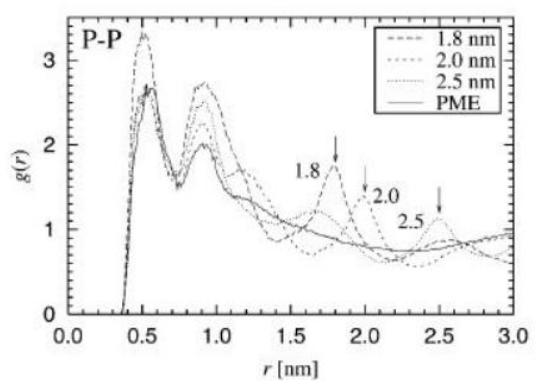
\includegraphics[scale=0.8]{artefact}
 \centering
 
\caption{Radial distribution function (RDF) $g(r)$ between the two
central atoms in the head-group of a molecule: Cutoff distances are indicated by arrows. from [ADD REFERENCE]}

\label{fig:artefact}

\end{figure}


As we can see in figure \ref{fig:artefact},  the radial distribution of the distance between two atom shows a peak, corresponding to the cutoff of the system. This shows that by using a cut-off technique we might see some artifacts.\\

So the two reasons we don't use a $\mathcal{O}(N^2)$ method is first because of its algorithmic complexity, and using some optimization techniques can also lead to artifacts that are detrimental to the accuracy of the simulation.



%-------------------------------------------------------------------------------------------


\section{Fourier Transform-Based methods}

In this section, we will explain techniques using periodic boundary conditions and Fourier transformation in order to compute the potentials and the forces of the particles.

\subsection{Ewald Summation}

This subset of techniques comes from a theoretical physics technique called the Ewald summation.

Using periodic boundary conditions, the potential $V$ of one particle of the system is:

\begin{equation}
	V = \sum_{n_x,n_y,n_z} \sum_{i}^{N} \sum_{j}^{N} \frac{q_i q_j}{r_{ij}}
	\label{periodicSum}
\end{equation}
where $n_x,n_y,n_z$ are the box index vector.\\

The equation (\ref{periodicSum}) is conditionally convergent and slow to converge. One technique discovered by Ewald is to split the potential in two absolutely convergent terms and one constant term:


If the system is neutral, ie. $\sum_{i=1}^N q_i = 0$, The idea is to split the potential the following way :

\begin{equation}
    V = \frac{1}{r} = \frac{f(x)}{r} + \frac{1 - f(x)}{r}
\end{equation}


\begin{equation}
    V = V_{\text{direct}} + V_{\text{reciprocal}}
\end{equation}

We want to choose $f$, so that $\frac{f(x)}{r}$ is quickly decaying and $\frac{1 - f(x)}{r}$ is as smooth as possible. In this decomposition $\frac{f(x)}{r}$  is as small as possible, even $0$ above a certain cut-off. Then, $\frac{1-f(x)}{r}$ is smooth enough so we can compute its Fourier transform with just a few $\overrightarrow{k}$ vectors. This gives a quick computation of the reciprocal space.

A good choice is often $f(x) = \text{erfc}(\alpha x)$, where $\alpha$ is called the splitting parameter, and $\text{erfc}(x) = \frac{2}{\sqrt{\pi}} \int_{x}^{+\infty}{e^{-t^2}\text{dt}} $\\

so we obtain the following potentials :\\

For the direct space :

\begin{equation}
   V_{\text{direct}} =  \frac{1}{2} \sum_{n_x,n_y,n_z} \sum_{i,j}^{N} q_i q_j \frac{\text{erfc}(\alpha r)}{r}
\end{equation}

and for the reciprocal space :

\begin{equation}
\label{Vrecip}
	V_{\text{reciprocal}} = \frac{1}{2 \pi V} \sum_{i,j}^{N} q_i q_j \sum_{n_x^*,n_y^*,n_z^*}\frac{\exp{-(\pi \overrightarrow{m}/\alpha)^2} +2\pi i \overrightarrow{m} \cdot (r_i - r_j)}{m^2}
\end{equation}

where $n_x^*,n_y^*,n_z^*$ are the vectors in the reciprocal space.\\


Once the electrostatic potentials are obtained, it is possible to differentiate the potentials to obtain the force on each particle.\\

let $p = (x,y,z)$ a coordinate of the system, then :


\begin{equation}
   \overrightarrow{F}_p^{\text{direct}} = \overrightarrow{\nabla}_p V_{\text{direct}} 
\end{equation}


so we have:

\begin{equation}
\label{ewaldDirect}
   \overrightarrow{F}_p^{\text{direct}} = q_i \sum\limits_{i=1,i\neq j}^N \sum\limits_{\textbf{n}} q_j \frac{(r_{ij,n})_p}{r_{ij,n}^3}
   \{\text{erfc}(\alpha (r_{ij,n}) + \frac{2\alpha}{\sqrt{\pi}} r_{ij,n} \exp(-(\alpha r_{ij,n})^2)\}
\end{equation}


\begin{equation}
\label{ewaldReciprocal}
   \overrightarrow{F}_p^{\text{reciprocal}} = \frac{2 q_i}{L} \sum\limits_{i=1,i\neq j}^N \sum_{n^* \neq 0} \frac{n_p^*}{n^{*^2}} \exp{(-(\frac{\pi m}{\alpha L})^2)}\sin{\frac{2\pi}{L} m \cdot r_{ij} }
\end{equation}

Equations \ref{ewaldDirect} and \ref{ewaldReciprocal} can then be used to compute the force on each particle by adding the direct space and the reciprocal space contribution.\\


\subsection{PME}

One way to improve this method is to compute the Fourier sum using the FFT (Fast Fourier Transform). This allows the algorithm to get a complexity of $\mathcal{O}(N\log N)$. There is different methods that are based on the Ewald summation, namely the \textbf{P3M} (Particle-Particle Particle-Mesh Method) or the \textbf{FFP} (Fast Fourier Poisson method). 

In our case, we will focus on the \textbf{PME} as it is the method currently used in GROMACS. \\

We remind that the potential for the reciprocal space $V_{\text{reciprocal}}$ is written in equation (\ref{Vrecip}):


\begin{equation*}
    V_{\text{reciprocal}} =\frac{1}{2 \pi V} \sum\limits_{i,j}^{N} q_i q_j \sum\limits_{\textbf{n}^*} \frac{\exp{-(\pi \overrightarrow{m}/\alpha)^2} +2\pi i \overrightarrow{m} \cdot (r_i - r_j)}{m^2}    
\end{equation*}



This equation can be rewritten as :

\begin{equation*}
    V_{\text{reciprocal}} =\frac{1}{2 \pi V} \sum\limits_{\textbf{n}^* \neq 0}^{N}  \frac{\exp{-(\pi \overrightarrow{m}/\alpha)^2}}{m^2}S(-\textbf{n}^* )S(\textbf{n}^* )
\end{equation*}

where $S(\textbf{n}^* )$ is defined as the Structure factor:

\begin{equation}
    S(\textbf{n}^* ) = \sum\limits_{k=1}^{N} {q_k \exp(2 \pi i \textbf{n}^* \cdot \textbf{r}) }
\end{equation}


The idea of the method is the following : In order to apply a FFT to the system, it is needed to "map" the positions of the charges on a grid of size $ p \times p $ . We will define the size of the Grid as the \textit{Fourier Spacing}. Let also define $\mathcal{F}(Q)$ the 3D FFT of $Q$. The charges $q_i$ are mapped to the grid using interpolation. 
Originally, Lagrange interpolation was used, but now a b-spline interpolation is used. The order of interpolation is called the \textit{PME Order}\\

then the Structure factor can be approximated as its FFT :

\begin{equation}
   S(\textbf{m}) \approx \widetilde{S}(\textbf{m}) = \mathcal{F}(Q)(\textbf{m})
\end{equation}

so the reciprocal energy can also be approximated by:

\begin{equation}
   V_{\text{reciprocal}} \approx \widetilde{V}_{\text{reciprocal}}   =\frac{1}{2 \pi V} \sum\limits_{\textbf{n}^* \neq 0}^{N}  \frac{\exp{-(\pi \overrightarrow{m}/\alpha)^2}}{m^2}\mathcal{F}(Q)(\textbf{m})\mathcal{F}(Q)(-\textbf{m})
\end{equation} \\

It can be shown that the complexity of such a system is $\mathcal{O}(N \log(N))$ which is a much bigger improvement compared to the $\mathcal{O}(N^2)$ complexity of the direct algorithm. However, one of its disadvantages is that it relies on a periodic sum, which is theoretically infinite. Furthermore, the algorithm doesn't scale well for large scale parallelism[REFERENCE ?], hence the need for a more scalable algorithm for the computations of electrostatic forces.



\section{Fast Summation methods}

    In the previous section we showed a method which allows to improve the speed of the computation. In this section, another algorithm will be explained, which has a complexity of $\mathcal{O}(N)$.\\
    
	\subsection{Mathematical preliminaries}
	
	Let's move back to the potential created by a charged particle as in (\ref{potential}),
	
	\begin{equation*}
	V = \frac{1}{d}
	\end{equation*}
	
	Let two particles $A(a,\alpha,\beta)$ and $B(r,\theta,\phi)$, separated by a certain distance $d$: The distance between the particles is $d = |a - r|$.
	We would like to achieve is to "factorize the addition", having a product of one function depending only on $a$ and one depending only on $r$.
	
	
\begin{figure}[H]
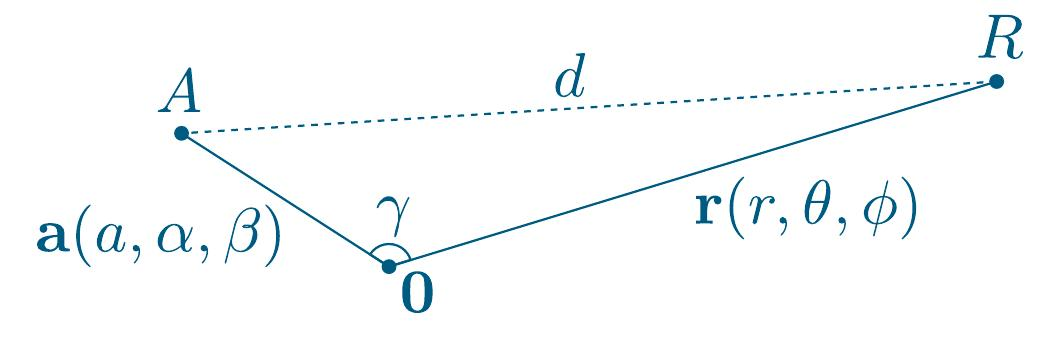
\includegraphics[scale=0.4]{distance}
 \centering 
\caption{Figure representing two particles $A(a,\alpha,\beta)$ and $B(r,\theta,\phi)$, separated by a certain distance $d$}
\label{fig:poster}
\end{figure}	
	
	
	The inverse distance can be written as :
	
	\begin{equation*}
		\frac{1}{d} = \frac{1}{|a-r|} = \frac{1}{\sqrt{a^2 + r^2}}
	\end{equation*}

	This distance can then written as a series :
	
	\begin{equation}
		\frac{1}{d} = \frac{1}{\sqrt{a^2 + r^2}} = \sum\limits_{l=0}^{+\infty} P_l(u)\mu^l
	\end{equation}
	
	
	where $\mu = \frac{a}{r}$ and $u = \cos{\gamma}$ . The $P_l(u)$ are the Legendre polynomials of degree $l$.
	
	with some manipulation as explained [ADD REFERENCE], we obtain : 
	
	\begin{equation}
	\frac{1}{|r - a|} = \sum\limits_{l=0}^{+\infty} \sum\limits_{m = -l}^{+l} \frac{(l-m)!}{(l+m)!} \frac{a^l}{r^{l+1}} P_{lm}\cos{(\alpha)}P_{lm}\cos{(\theta)}e^{-im(\beta - \alpha)}
	\end{equation}
	
	in order to approximate the scheme, we can truncate the series to a certain order $p$, we call this order the \textbf{multipole order}
	
	\begin{equation}
	\frac{1}{|r - a|} \simeq \sum\limits_{l=0}^{\textcolor{red}{p}} \sum\limits_{m = -l}^{+l} \frac{(l-m)!}{(l+m)!} \frac{a^l}{r^{l+1}} P_{lm}\cos{(\alpha)}P_{lm}\cos{(\theta)}e^{-im(\beta - \alpha)}
	\end{equation}
	
	We can now rewrite the summation the following way :
	
		\begin{equation}
	\frac{1}{|r - a|} \simeq \sum\limits_{l=0}^{p} \sum\limits_{m = -l}^{+l}
	\underbrace{\frac{a^l}{(l+m)!} P_{lm}(\cos(\alpha))e^{-im\beta}} _{O_{lm}(\textbf{a})}
    \underbrace{\frac{(l-m)!}{r^{l+1}} P_{lm}(\cos(\theta))e^{+im\phi}} _{M_{lm}(\textbf{r})}
	\end{equation}
	%and ${M_{lm}(\textbf{r})$
	hence,
	
		\begin{equation}
	\frac{1}{|r - a|} \simeq \sum\limits_{l=0}^{p} \sum\limits_{m = -l}^{+l}
	{O_{lm}(\textbf{a})}
    {M_{lm}(\textbf{r})}
	\end{equation}
	
	
	We have shown that it is possible to "factorize" the inverse of the the distance $\frac{1}{d}$ so we can obtain two independent terms for two independent particles ${O_{lm}(\textbf{a})}$ and ${M_{lm}(\textbf{r})}$ 


	We can then define the multipole moment $\omega_{lm}(q,\textbf{a}) = q O_{lm}(\textbf{a})$ and the Taylor-like moment $\mu_{lm}(q,\textbf{r}) = q M_{lm}(\textbf{r})$
	
	Then, it is possible to show that it is possible to obtain the following "bipolar expansion" for two particles associated with two different origins :
	
    \begin{equation}
    \frac{1}{|\textbf{a}_1 - \textbf{a}_2 + \textbf{R}|} = 
    \sum\limits_{l=0}^{+\infty}
    \sum\limits_{j=0}^{+\infty}
    \sum\limits_{m=-l}^{+l}
    \sum\limits_{k=-j}^{+j}
    (-1)^j \cdot O_{lm}(\textbf{a}_1) \cdot M_{l+j,m+k}(\textbf{R}) \cdot O_{jk}(\textbf{a}_2)
    \end{equation}



	\begin{figure}[H]

    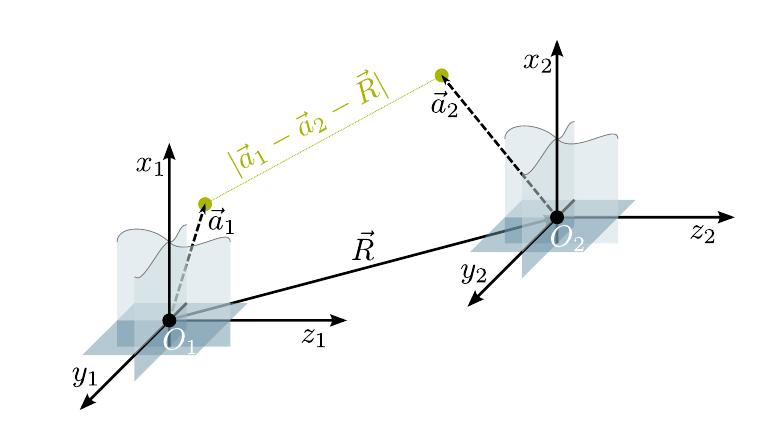
\includegraphics[scale=0.7]{bipolar}
    \centering 
    \caption{Scheme of two particles expanded according to two different origins [from ADD REFERENCE]}
    \label{fig:bipolar}
    \end{figure}




	
	\subsection{Workflow of the algorithm}
	
	Once some Mathematical preliminaries are set, it is possible to explain the workflow of the Algorithm.
	
	\subsubsection{Spliting the Space}
	
	The first step of the scheme is to split the space in order to generate different groups. The idea is to recursively split the space in eight octants, created the so-called structure of an \textit{octree}. So the number of boxes is $8^{D-1}$, where $D$ is the depth of the oct-tree.
	
		
	
	\begin{figure}[H]
    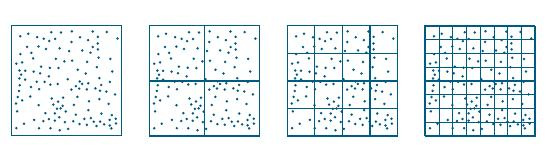
\includegraphics[scale=0.9]{BoxDepth}    
    \centering 
    \caption{Example of a division of the space in boxes. The following example is in 2D so the structure of the space is a \textit{quadtree}.}    
    \label{fig:depth}
     \end{figure}
	
    
    The number of subdivisions is called the \textit{depth} $D$. For example, in figure \ref{fig:depth}, we can observe from left to right the depths $0,1,2$ and $3$.
    
    It is then possible to assign each particle of the simulation to the boxes of lowest depth.
    
	\subsubsection{Defining a Separation Criterion}
	
	For the further Computations it is needed to define a separation criterion $ws$: It is the $ws^{th}$ next neighbors of a given box. Two boxes A and B are called \textit{next neighbors} is they are at the same level and box B is enclosed by a box of size $(2 ws + 1)^3$ around the center of A 
	
	
	
	
	\begin{figure}[H]
    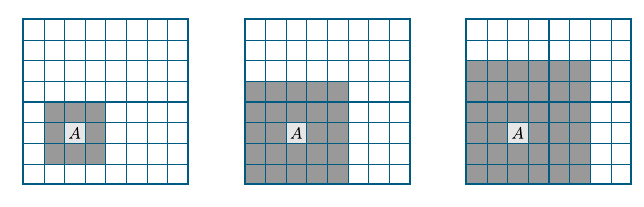
\includegraphics[scale=0.7]{separation}    
    \centering 
    \caption{Example of the influence of the separation criterion $ws$ for a given box $A$, from left to right, $ws = 1,2,3$.}    
    \label{fig:depth}
     \end{figure}
	
		This separation criterion divides the space into two parts. If two particles are close so they are in the same grey space as defined figure (\ref{fig:multipole}), then, they will interact via a direct $\mathcal{O}(N^2)$ coulombic interaction ; else they will interact via using the FMM Method.
	
	It is most of the time not possible to set the separation criterion $ws$ to 0, as the multipole expansion might overlap. Using a bigger ws means that the order of the multipole expansions need to be less important for the same precision, however this will increase the number of direct $\mathcal{O}(N^2)$ operation, which are  more computationally expensive.       
    
    
    \subsubsection{PASS 1 : Computing the Multipole moments}
    
    Once every particle is assigned to its box, we will compute the multipole moment $\omega_{lm}^j$ of each box.
    
    \begin{equation}
    \omega_{lm}^{j}(q,\textbf{a}) = q^j a_j^l \widetilde{P}_{lm}(\cos(\alpha_j))e^{-im\beta_j}
    \end{equation}
%
Then each multipole order can be moved to the Center of the box using the so-called $M2M$ (Multipole to Multipole) operator:    
    
    \begin{equation}
    \omega(\textbf{a} + \textbf{b}) = \sum\limits_{j=0}^{k} \sum\limits_{k=-j}^{j} \omega_{jk}(\textbf{a}) O_{l-j,m-k}(\textbf{b})
    \end{equation}

   $O_{l-j,m-k}(\textbf{b})$ is called the $M2M$ operator
   
   \begin{figure}[H]
   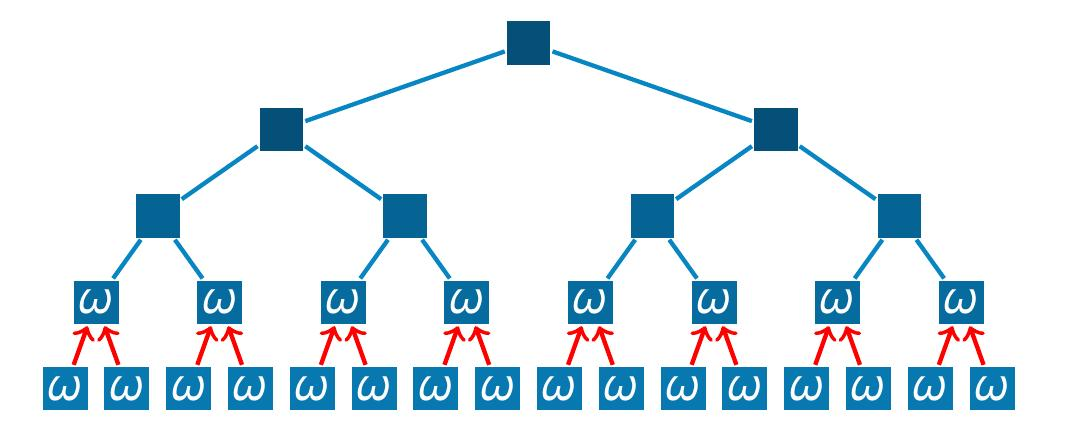
\includegraphics[scale=0.4]{ShiftMultipole}
    \centering 
    \caption{Example in 1-D showing the shifting of the multipole moments using the M2M operator. }
    \label{fig:multipole}
   \end{figure}
   
   
   	\subsubsection{PASS 2 : Transforming distant expansions into multipoles}
   	
   	Now it is possible to transform distant expansions (above the separation criterion) $\omega_{lm}$ into a Taylor-like moment $\mu_{lm}$. This transformation is done over at most 189 boxes. This transformation is applied for each depth of the tree.  
   	
   	
 \begin{figure}[H]
 	\label{fig:M2L}
   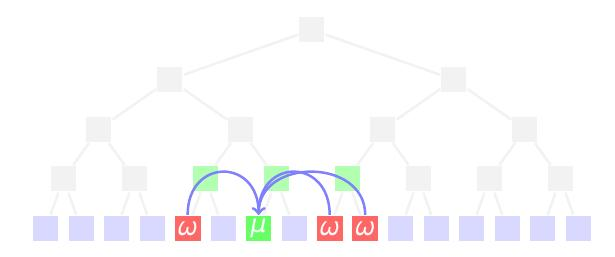
\includegraphics[scale=0.8]{transformExpansions1}
    \centering 
    \caption{Example in 1-D showing the transformation of distant expansions into multipoles}
    
   \end{figure}
   
	In order to compute this transformation, two different rules have to be applied:
	
	\begin{itemize}
	
	\item The first rule is to take the non-separated parent boxes, as showed sub-figure (a) below.
	\item Then the children of the parent box are selected, taking into account the separation criterion for the child boxes.
	
	\end{itemize}	   
   
	 
 \begin{figure}[H]
   \subfloat[First, the parents of the box are chosen] {\label{fig:parentBox} 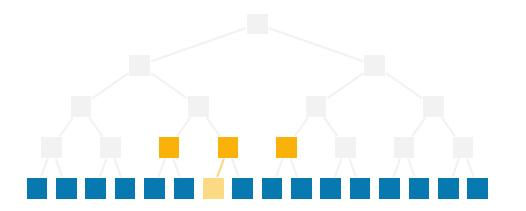
\includegraphics[scale=0.6]{transformExpansions2}}   
   \subfloat[Then, then children of the parents are chosen. Then the separation criterion can apply] {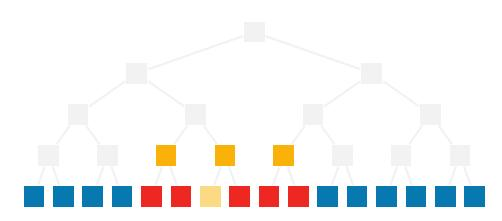
\includegraphics[scale=0.6]{transformExpansions3}}
    \centering 
    \caption{Interation Rules for the transformation of the multipole expansions}
    \label{fig:multipole}
   \end{figure}   
   
	  Mathematically speaking, the transformation from multipole expansions to multipole moments is given using the  M2L (Multipole to Local) Operator
	  
	  \begin{equation}
	  \mu_{lm}(\textbf{b} - \textbf{a}) = \sum\limits_{j = 0}^{+\infty} \sum\limits_{k=-j}^{j}
	  M_{j+l,k+m}(\textbf{b}) \cdot \omega_{jk}(\textbf{(a)})
	  \end{equation}
   
   	where $M_{j+l,k+m}(\textbf{b})$ is the M2L operator : It allows to exchange, as figure (\ref{fig:M2L}) shows, information between boxes of the same level.

\subsubsection{PASS 3 : Shift Taylor-Like expansions down the tree}

Once the local $\mu_{lm}$ expansions are computed, the expansion have to shifted to the lowest level of the tree using the L2L (Local to Local) operator.

	\begin{figure}[H]
	\label{fig:L2L}
   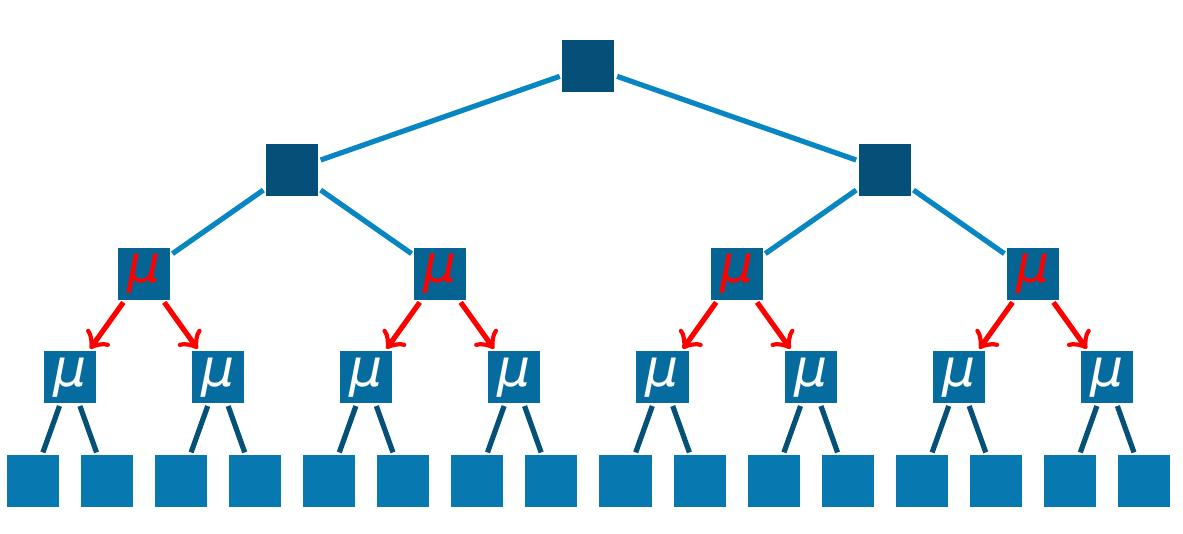
\includegraphics[scale=0.4]{L2L_1}
    \centering 
    \caption{Example in 1-D showing the shifting of the local moments using the L2L operator. }
    
   \end{figure}
    
 	This shift operation is done by the following formula :
 	
 	  \begin{equation}
	  \mu_{lm}(\textbf{r} - \textbf{b}) = \sum\limits_{j = l}^{p} \sum\limits_{k=-j}^{j}
	  O_{j-l,k-m}(\textbf{b}) \cdot \mu_{jk}(\textbf{(a)})
	  \end{equation}
 
 		where $O_{j-l,k-m}(\textbf{b})$ is the L2L operator : It allows to exchange, as figure (\ref{fig:M2L}) shows, information between levels downwards.
 		
 \subsubsection{PASS 4 : Computing forces and Energies}
 
 
 After PASS 3, we have at the lowest level both the multipole expansion as well as the local expansion. 
 
\begin{figure}[H]
	\label{fig:farfield}
   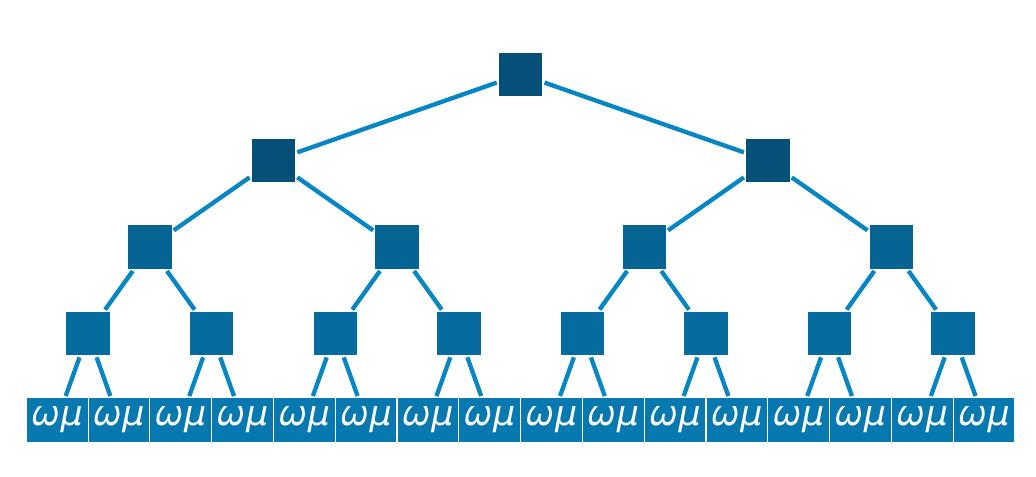
\includegraphics[scale=0.5]{farfield}
    \centering 
    \caption{Situation after PASS 3 }
    
   \end{figure} 
   
   Then we have everything to compute the far-field contribution for the forces or the potentials of the system.\\
   
   So we have for the Electric Field :
      
   \begin{equation}
   E_{FF} = \sum\limits_{l=0}^{p} \sum\limits_{m=-l}^{+l} \mu_{lm}(\textbf{r}) \omega_{lm}(\textbf{a})
   \end{equation}
   
   For the Potential :
 
 	\begin{equation}
   \Phi_{FF} = - \sum\limits_{l=0}^{p} \sum\limits_{m=-l}^{+l} \mu_{lm}(\textbf{r}) \nabla_{\textbf{a}_i}[a_i^l \widetilde{P}_{lm}(\cos\alpha_i)e^{-im\beta_i}]
   \end{equation}
   
   and for the Force :
   
   \begin{equation}
   \textbf{F}_{FF} = - \sum\limits_{l=0}^{p} \sum\limits_{m=-l}^{+l} \mu_{lm}(\textbf{r}) \nabla_{\textbf{a}_i}[a_i^l \widetilde{P}_{lm}(\cos\alpha_i)e^{-im\beta_i}]
   \end{equation}
   
 Then the near-field contribution can be easily computed : 

 

\chapter{Comparing FMM and PME accuracy}

    In this chapter I will more precfisely explain my work done in the Lab, which consisted in comparing the PME methods, which is for example used by gromacs, and the FMM mnethod, used by a solver made between the Julich Forschungszentrum and the Max Planck Institute for Biophysics in Göttingen.

    In will first explain for Gromacs work and then 


\section{Presentation of GROMACS}

    GROMACS (GROningen MAchine for Chemical Simulations) is a simulation software used for Molecular dynamics. It was originally developed in the Biophysical Chemistry department of University of Groningen but it is now develloped arround the world. GROMACS is made to be as fast as possible using all possible techniques to improve its performance (MPI, GPU computing) 
    
   
	\subsection{Structure of a File}
	
	 The program is used  by modifying text files that giving information on the structure of the system that has to be simulated and the parameters of the simulation. The files are the following 
	 
	\begin{itemize}
	
	\item The *.pdb file are the \textit{Protein DataBank} file : In this file is denoted the position and the type of the particles of the system. It also gives the size of the simulation box

	\item The *.top files (namelt \textit{topoloy} files) are the file where the properites of the atoms are defined. These properties are for example the charge, the Van-der-Waals parameters or the binding forces of the system. This configuration is often done with force field files such as AMBER or CHARMM
		 
	\item The *.mdp files are defining the physical and computational parameters of the simulation. It is defining the methods used for the simulation. In our case we are mostly interested in the electrostatics part of the computation ; it is then possible to select the method (PME or Cut-Off methods) and the parameters for the PME
	
	\end{itemize}
		
	\subsection{PME parameters}
	
	In this paragraph I will explain the parameters it is possible to play with:
	
	\begin{enumerate}
	

	\item[\textbf{CutOff}] The first parameter is the CutOff : It allows to set the Cut-Off radius for the Cut-Off method, but it also sets the difference between the direct part and the reciprocal part in the PME method
	
	\item[\textbf{Fourier Spacing}] The other important parameter is the fourier spacing. I remind that in the PME method a 3D FFT is done in order to compute the energies and the forces of the system. The FFT is so computed on a grid : The dimension of the grid is given by the \textit{Fourier Spacing} parameter.
	
	\item[\textbf{PME Order}] The PME order gives the order of the interpolation. For instance, PMEorder$= 4$ corresponds to a cubic interpolation. 		
	
	\end{enumerate}
	
	\subsection{Command to launch a GROMACS simulation }	
	
The workflow to laumch a GROMACS Simulation is the following : 



First generate a .tpr binary file conaining all the information about the simulation. The file is processed using the \textit{grompp} (Gromacs Preprocessor). The command is :


{\centering\tt {grompp -f mdpfile \\
	 -p topFile.top \\
	 -c pdbFile.pdb \\
	 -o tprFile.tpr \\ 
 }}

\vspace{5mm}
where the input files are the *.mdp , *.top and *.pdb (Respectively properties of the Simulation, of the atom, and the opsition of the At and contains arroundoms). The *.tpr file ris the output file.

It is then possible to run the simulation using the program mdrun, which as its name stands, runs the md simulation. A possible example is :

{\centering\tt { mdrun -s tprfile.tpr \\
				 -ntomp = 4  			\\		
				 -ntmpi = 4				 \\
				 -nsteps= 0     		  \\  
 }}
 
\vspace{5mm}

Where the .tpr File is now the input file, containing everything about the simulation, -nsteps is the number of time steps needed (In the case of this Intership, no time intergration is needed as just the forces are required). It is also possible to choose the number of CPU cores needed for the simulation (Using MPI and OpenMP).

\section{Presentation of fmsolvr}	

	The software used to compute the electrostatic forces with the FMM is not gromacs (at least not for the moment). It is develloped by both the Max-Planck Institut for Biophysical Chemistry and the Jülich Forschungszentrum . In the following chapters, we will call this code \textit{fmsolvr}. 
	
	The codebase is mostly written in C++.  There exists several git branches for the program, allowing different versions of the system.	
The First version is a sequential version, which is the "basic" version of the FMM code . There also exists a version which allows periodic boundary conditions : We will use this version a lot as we need to campare it to the PME, which, by construction, uses periodic boundary conditions.	

The input file, is a *.hpp file containing 4 arrays of size $N$, where $N$ is the number of atoms in the simulation : one charge array $q$ , and three array $x,y,z$ for the positions of the atoms.

\subsection{FMM Parameters}

The simulation can be launched using the following command : 

{\centering\tt { DEPTH=\${DEPTH}  MULTIPOLEORDER=\${MULTIPOLEORDER}  WS=\${WS} \\ 
OPENBOUNDARY=0 UNITBOX=\${UNITBOX} CENTER=c \\
./fmmtest \$inputFile.qxyz \$outputFile.dat \\					
 }}

The environment variables are the following :

\begin{description}
\item[DEPTH] The maximal subdivision of the space : if DEPTH=n the space will be divided in $8^{n}$ boxes.

\item[MULTIPOLEORDER] The Order of truncation in a the series, for instance :
\begin{equation*}
	\frac{1}{|r - a|} \simeq \sum\limits_{l=0}^{\textcolor{red}{p}} \sum\limits_{m = -l}^{+l} \frac{(l-m)!}{(l+m)!} \frac{a^l}{r^{l+1}} P_{lm}\cos{(\alpha)}P_{lm}\cos{(\theta)}e^{-im(\beta - \alpha)}
	\end{equation*}15:20 - 16:00 - Gautier VAILLANT
	
	where the multipole order is the red \textcolor{red}{p} in the first summation.
	
	
\item[WS] This gives the separation criterion $ws \geq 1$, which separates the far-field computation from the near space.

\item[OPENBOUDARY] if OPENBOUNDARY = 0, periodic boundary conditions will be used, if OPENBOUNDARY=1, then openbondaries will be used.

\item[UNITBOX] Gives the size of the simulation box (in nm.

\end{description}
 	
\section{Making GROMACS and fmsolvr comparable}	

The first part, if we want to make the PME and the FMM comparable, is to use the same simulation for both programs, hence requiring coding some tools transforming a GROMACS-compatible file to fmsolvr-compatible one. Then, we saw that the results we obtained weren't good enough as one system was using some dipole correction, so we needed to implements the dipole correction to the FMM system.

\subsection{File manipulation}

In this section will be explained the file modifications needed in order to have the simulations comparable on both systems.

\subsubsection{Making GROMACS only compute electrostatics forces}

In this Internship we just want to compute the electrostatic forces on our system. However, what we obtain in the GROMACS output file is the sum of all forces on each atom. These forces may include forces such as for instance Lennard-Jones potentials.
($V_{LJ} = 4\epsilon [(\frac{\sigma}{r})^12 - (\frac{\sigma}{r})^6] $). 

So the first thing to do is to modify the topology file (*.top), so there is no more Lennard Jones potential at all ; this snippet is added to the *.top file:


{\centering\tt {
[ atomtypes ]\\
type atnum         mass   charge ptype           sigma  epsilon\\
  CLA    17    35.450000    0.000  A  0.000000000000  0.00000\\
  SOD    11    22.989770    0.000  A  0.000000000000  0.00000\\
}}

In the expression of the potential, we set $\epsilon = 0$ and $\sigma = 0$, so it gives $V_{LJ} = 0$. So we have modified the files such that there is only the electrostatic interaction at play in the simulation.

\subsubsection{Assure compatibility between *.qxyz and *.pdb files}

The next thing to do is to have the same simluation system for both methods : So I needed to make a few scripts to transform a *.pdb file in a *.qxyz or a *.hpp file.

The scripts are written in python, the workflow is the following:

{
	\centering 
	{
	
	  *.hpp $\xleftarrow{\tt{qxyz2hpp.py}}$  *qxyz $\xrightarrow{\tt{qxyz2gromacs.py}}$ *.pdb	
	}
}

So it is now possible to move the positions of the atoms one software to another software. (PME to FMM or FMM to PME)

\subsubsection{Output positions and forces to a Text file for GROMACS}

The last preliminary thing to do is to make the GROMACS Simulation print the positions and the forces in an easy and detailled way. We decided to modify the Gromacs code to add after the so-called {\tt{do\_force(...)}} function, which computes the forces for the system, a routine that prints the force as well as the positions in order to be
 easily used afterwards. 

\section{First Comparisions and Dipole Correction}

\subsection{Silicamelt Simulation}

The first thing we did afterwards it to take a good precision for both methods and compare the forces.

The model we are using is called the "Silicamelt" system which is a system composed of $SiO_2$ atoms : It is a system compased of about 100000 atoms, the silicon atoms (Si) have a $+2.4e$ charge and the Oxygen has a charge of $-1.2e$.
The size of the simulation box is $124.120$ nm.

The parameters for the PME simulation are cutoff=1.2nm, PME order=12 and fourier spacing=0.015 nm. 

The paramerters for the FMM are : Depth=4, Multipole Order=40, and WS(Separation Criterion) =4. The simulations is done with periodic boundaries \\

The relative error is computed the following way, assuming the PME is more accurate than the FMM:

\begin{equation}
	error_{\text{relative}} = \frac{F_{FMM} * F_{PME}}{F_{PME}}
\end{equation}

Then the following histogram can be plotted:

\begin{figure}[H]

   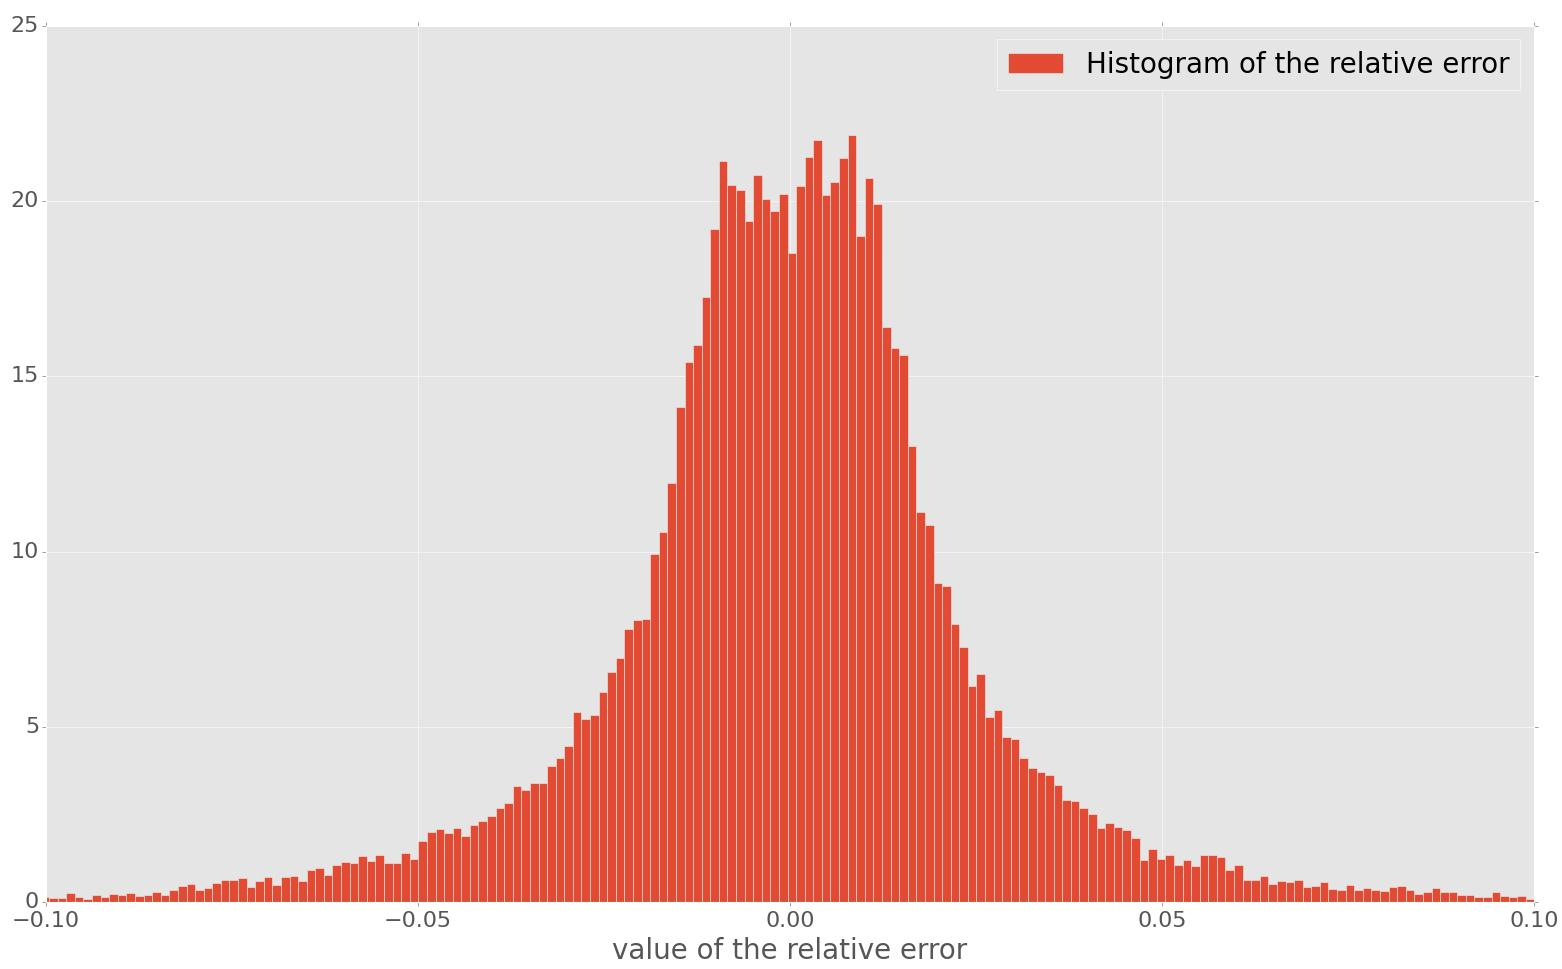
\includegraphics[scale=0.25]{hist_nocorrection.jpeg}
    \centering 
    \caption{Histogram representing the relative error for a silicamelt simulation : The histogram is computed before any diple correction.}    
   \end{figure}   


	\begin{figure}[H]
	   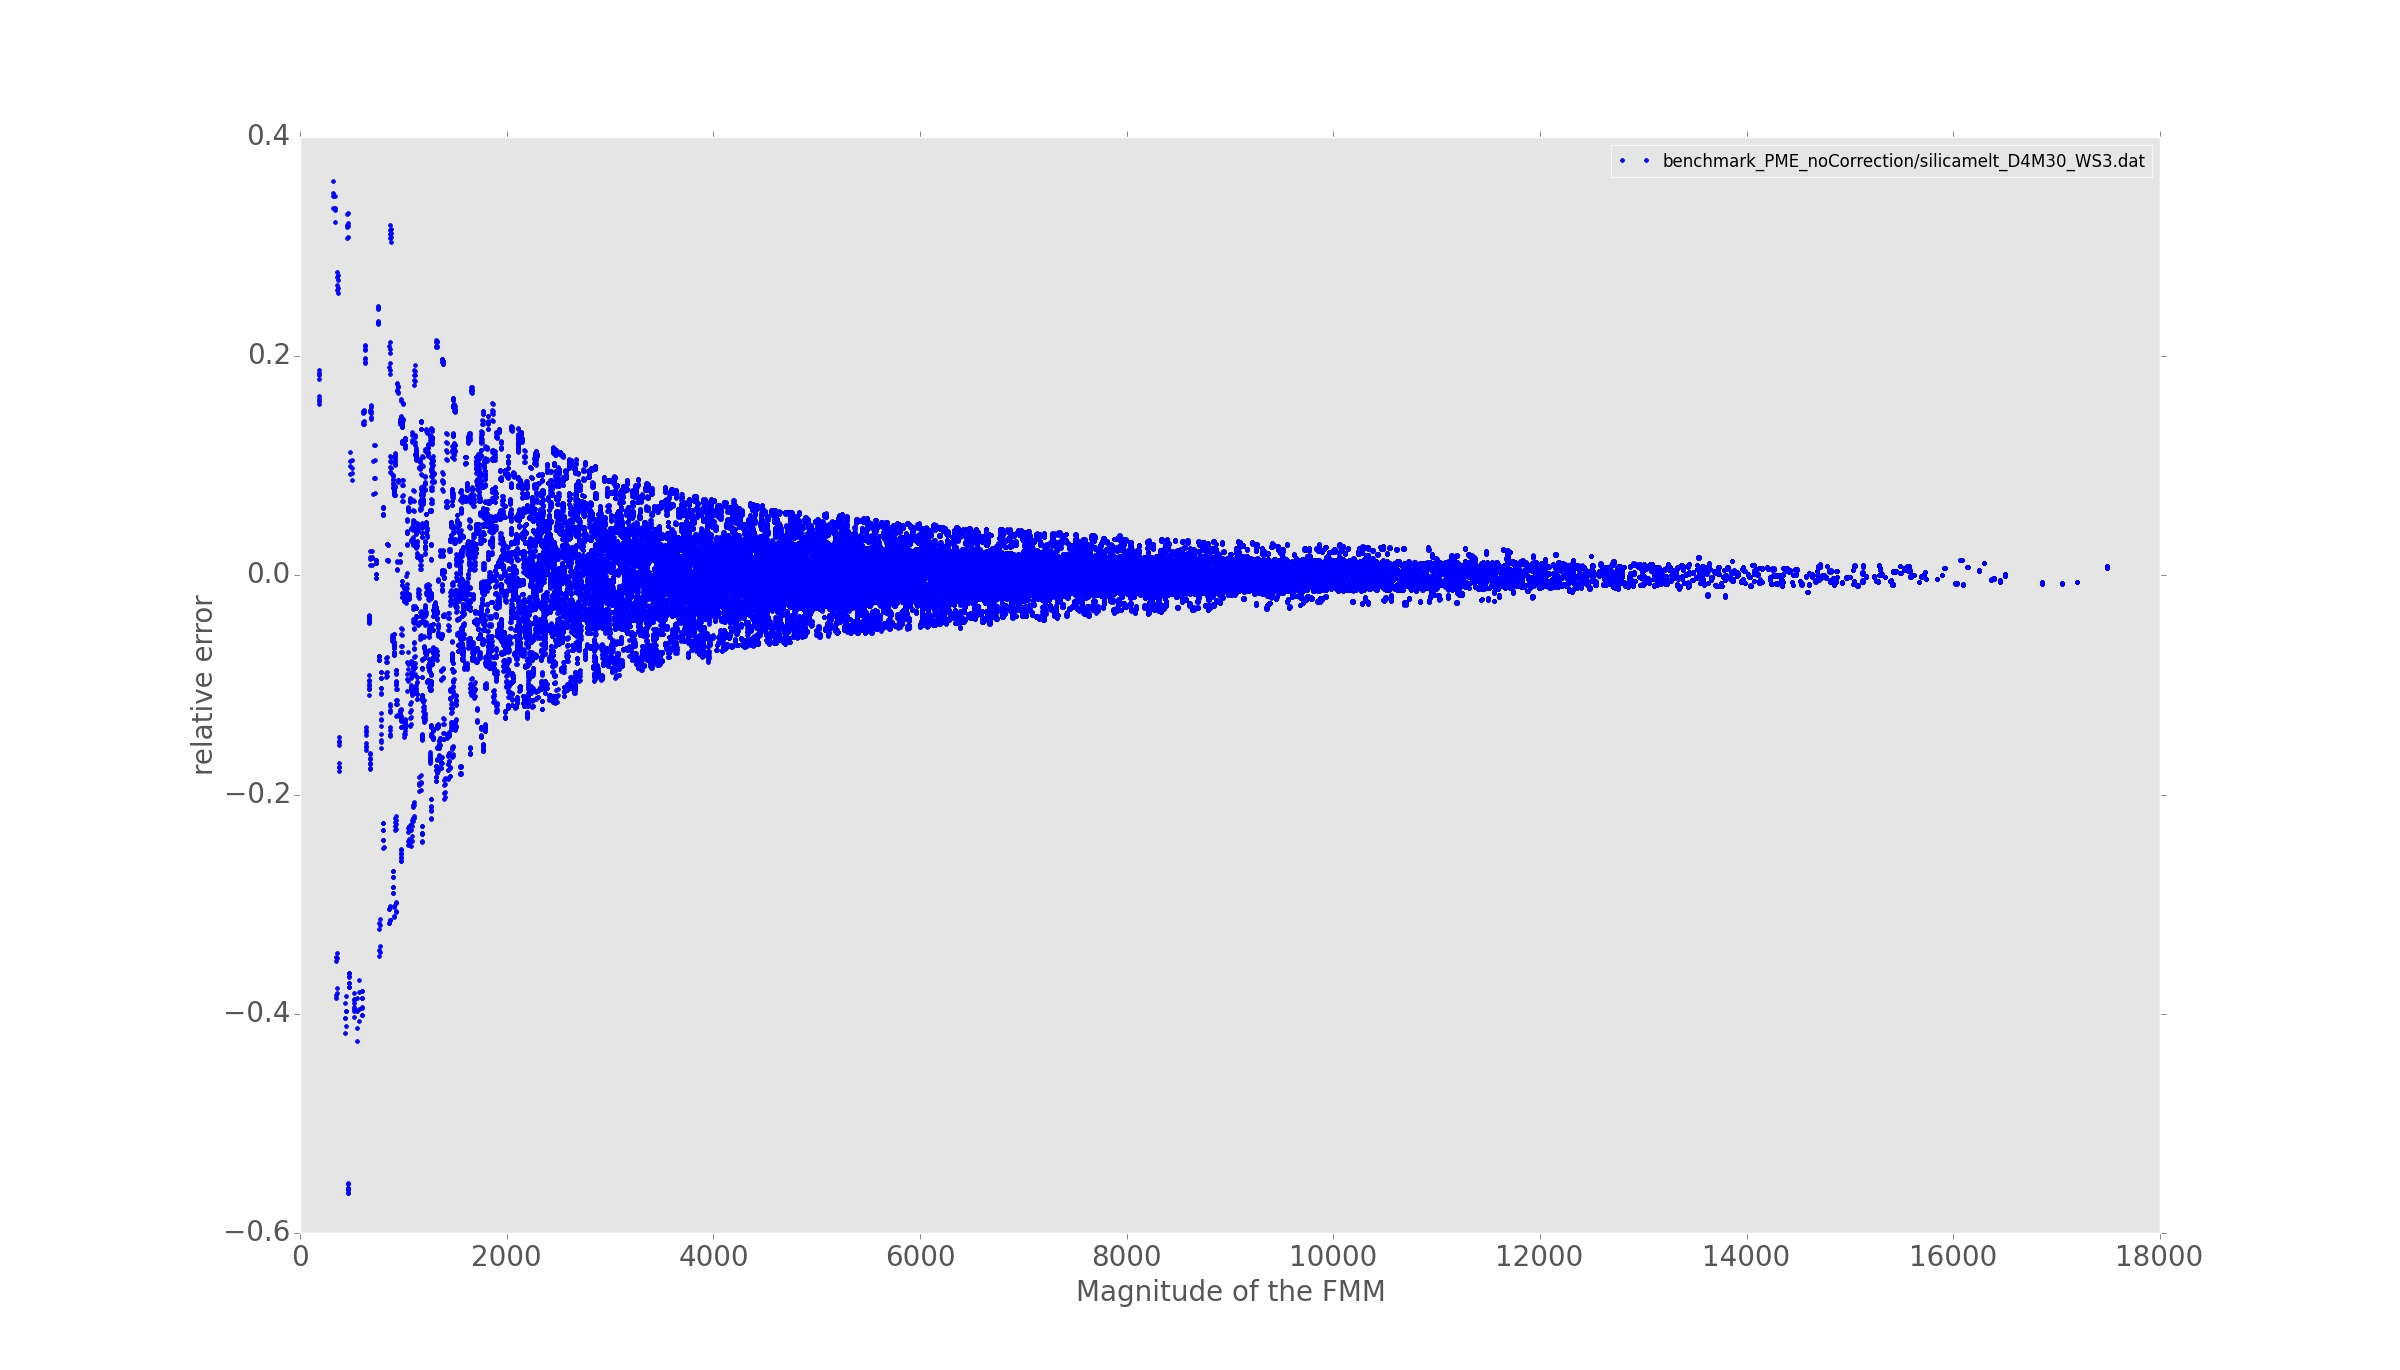
\includegraphics[scale=0.2]{magErr_noCorrection.jpeg}
    \centering 
    \caption{Figure representing the Magnitude of the force in the x-axis and the  error in relative error in the y-axis. It is possible to see that the biggest errors are when the magnitude of the force is smaller.}    
   \end{figure}  


	Some statistical information about the distribution gives us a maximum error of about 56.35\%, this maximum error is much bigger than expected and is therefore not acceptable.\\
	
	If we study the distribution of errors according to the magnitude of system we can see that the biggest errors are some smaller magnitudes.
	

	
\subsection{Dipole correction}
\subsubsection{Study of a two-particle system}
	In order to understand these big errors, we first decided to study how 2 particles behave. Then if the errors are small enough, it is possible to move to bigger systems.
	
The hypothesis is that the dipole moment may be corrected in one system and not in another system. So the idea is to take two particles, one positively charged and the other negatively charged ; the two particles will form a dipole, namely : 

\begin{equation}
	\vec{p} = q \vec{d}
\end{equation}	
	where $\vec{d}$ is the displacement vector pointing from the negative charge to the positive charge. 
	
	Then we can vary the distance between the two particles, compute the force using both the FMM method and the PME method and compare the force.
	
	
	\begin{figure}[H]
	   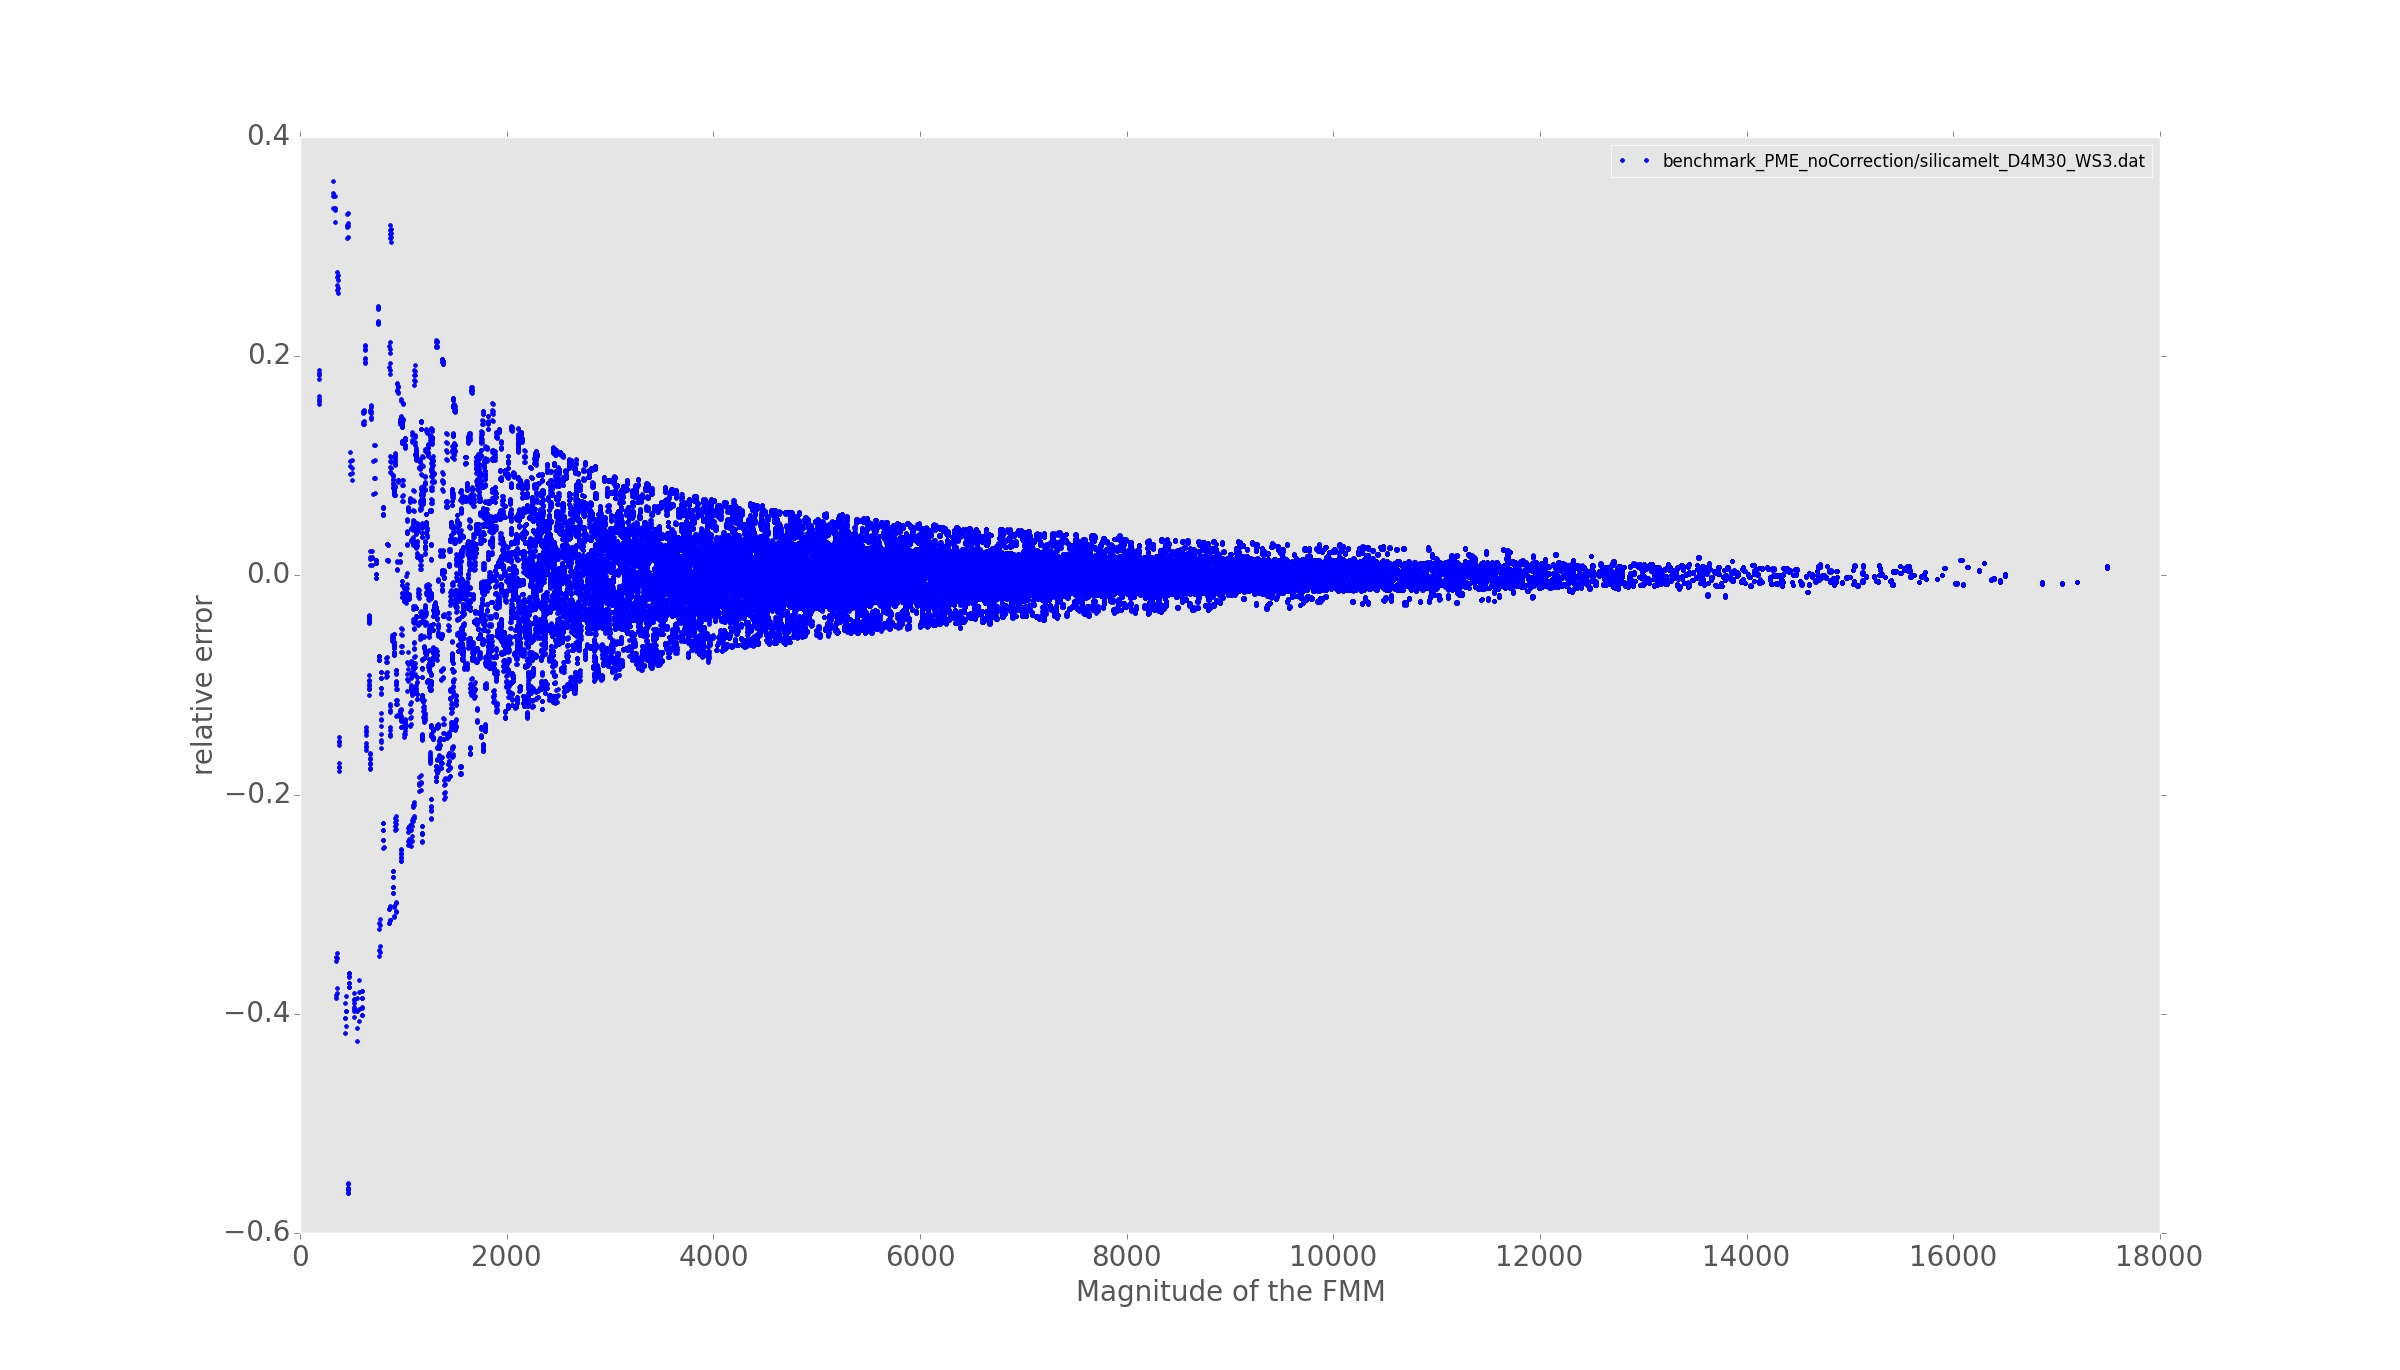
\includegraphics[scale=0.2]{magErr_noCorrection.jpeg}
    \centering 
    \caption{Figure representing the Magnitude of the force in the x-axis and the  error in relative error in the y-axis. It is possible to see that the biggest errors are when the magnitude of the force is smaller.}    
   \end{figure}  
	
	
	
	
\subsubsection{Back to the silicamelt simulation}

\section{Comparing with an analytical solution : the NaCl system}

\subsection{Generating the system}
\subsection{Error plots}




\nocite{*}
\bibliographystyle{plain}
\bibliography{biblio} 

\begin{appendices}
\chapter{Glossary}
\chapter{Structure of Gromacs files}
The contents...
\end{appendices}



























\end{document}